QR codes technology has been employed to identify distincts \textbf{points of interest (POIs)} within the indoor environment. \textit{POIs} represent specific locations that the users may find useful or interesting, such as bathrooms or lecture rooms.

To implement our application effectively, we have utilized two types of QR codes: \textit{floor} QR codes and \textit{door} QR codes. The \textit{floor} QR codes have been positioned on the ground in front of each POI, allowing users to scan them while walking. On the other hand, the \textit{door} QR codes have been placed on the doors of the respective POIs. These QR codes serve as markers for users to easily find the wanted POI.

For this purpose, we adopted the CameraX API for handling the camera and Google's ML Kit API for analyzing the taken images.


\subsubsection{CameraX and ML Kit}

\textbf{CameraX} is an Android Jetpack library, built to help make camera app development easier. 
It provides a consistent, easy-to-use API that works across the vast majority of Android devices.\cite{android:camerax:overview}
One of the main strengths of CameraX is its ease of use: in fact, the API emphasizes \textit{use cases}, which allows the developer to focus on the task that needs to be done instead of managing device-specific nuances.\cite{android:camerax:analyze}
In particular, CameraX offers a pre-built \textit{Image Analysis} use case, which provides CPU-accessible buffers on which can be performed image processing, computer vision, or machine learning inference.\cite{android:camerax:analyze}

\textbf{ML Kit} is a mobile SDK (Software Development Kit) provided by Google that enables developers to integrate\textit{ machine learning capabilities} into their Android and iOS applications. 
ML Kit offers a range of ready-to-use APIs and pre-trained models, simplifying the process of incorporating machine learning functionality into mobile apps without requiring extensive machine learning expertise.\cite{android:mlkit:overview}

In particular, ML Kit offers a \textbf{barcode scanning API}, which allows the developer to read data encoded using most standard barcode formats, such as \textit{QR codes}.\cite{android:mlkit:barcode}
Its key capabilities are the following:
\begin{itemize}
    \item Out-of-the-box support for \textit{most standard barcode formats}, both linear and 2D.
    \item Automatic \textit{format detection}.
    \item Automatically parses \textit{structured data} stored in the barcode.
    \item Recognizes and scans barcodes regardless their \textit{orientation}.
    \item Runs locally on the \textit{device}.
\end{itemize}

Android offers a library (\path{androidx.camera.mlkit.vision}) which provides a \textbf{seamless integration} between CameraX and Google's ML Kit\cite{androidx.camera.mlkit.vision}, which allows to directly forward frames generated in the \textit{Image Analysis} use case to the \textit{barcode scanner}.\cite{androidx.camera.mlkit.vision.MlKitAnalyzer}



\subsubsection{QR codes deployment}

As mentioned earlier, we implemented two distinct types of QR codes: floor QR codes and door QR codes.

The application utilizes \textbf{floor QR codes} to alert users about nearby points of interest. 
To ensure that QR codes are not missed by the walking user, we decided to position \textit{horizontal strips} of QR codes across the entire width of the hallway, as shown in Figure \vref{fig:floor-qr-codes}. 
This design choice is inspired by the \textit{NavCog system}\cite{indoor-navigation-qr-codes}, which achieved error-free scanning of QR codes for indoor navigation.

\begin{figure}[H]
    \centering
    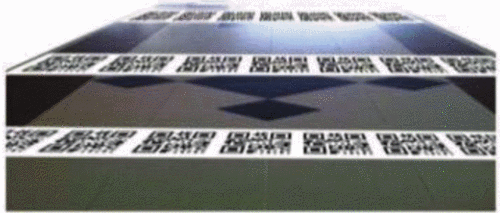
\includegraphics[width=\columnwidth]{chapters/architecture/images/ground-qr-codes.png}
    \caption{Example of intended arrangement of QR codes placed on the ground.\cite{indoor-navigation-qr-codes}}
    \label{fig:floor-qr-codes}
\end{figure}

To ensure effective scanning, the user is required to hold their smartphone device \textit{horizontally} and direct the camera towards the ground. Once the application successfully scans a QR code on the floor, it immediately provides an audible notification to inform the user about the nearby presence of the corresponding point of interest.

As depicted in Figure \vref{fig:multiple-qr-codes}, Google's ML Kit library effectively distinguishes between \textit{different QR codes} within the same image frame. 
Our application is designed to analyze and process \textit{only one of the detected QR codes at a time}, so, since the QR codes in the same strip contain the same value, the presence of multiple QR codes in close proximity will not cause any interference or confusion in its functionality.


\begin{figure}[H]
    \centering
    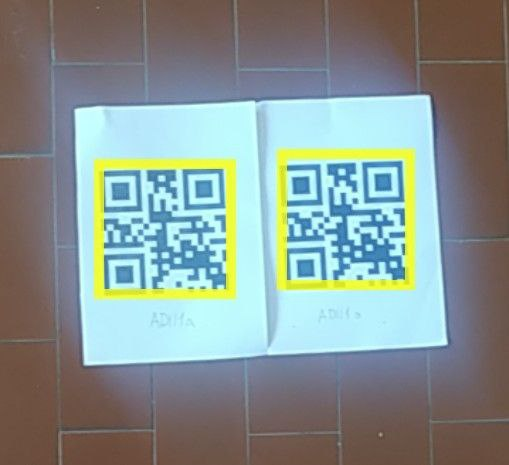
\includegraphics[width=0.6\columnwidth]{chapters/architecture/images/multiple-qr-codes.jpg}
    \caption{Screenshot taken from the Android app which shows how the ML Kit library is able to discern different QR codes in the same frame.}
    \label{fig:multiple-qr-codes}
\end{figure}


On the other hand, the \textbf{door QR codes} are employed to specify the \textit{exact} location of a point of interest (Figure \vref{fig:door-qr-codes}). Once the user locates the relevant floor QR code, which indicates the nearby presence of the point of interest, they should hold their smartphone in a \textit{vertical} position, so that the application can scan the surrounding environment and determine the precise direction in which the point of interest is situated.


\begin{figure}[H]
    \centering
    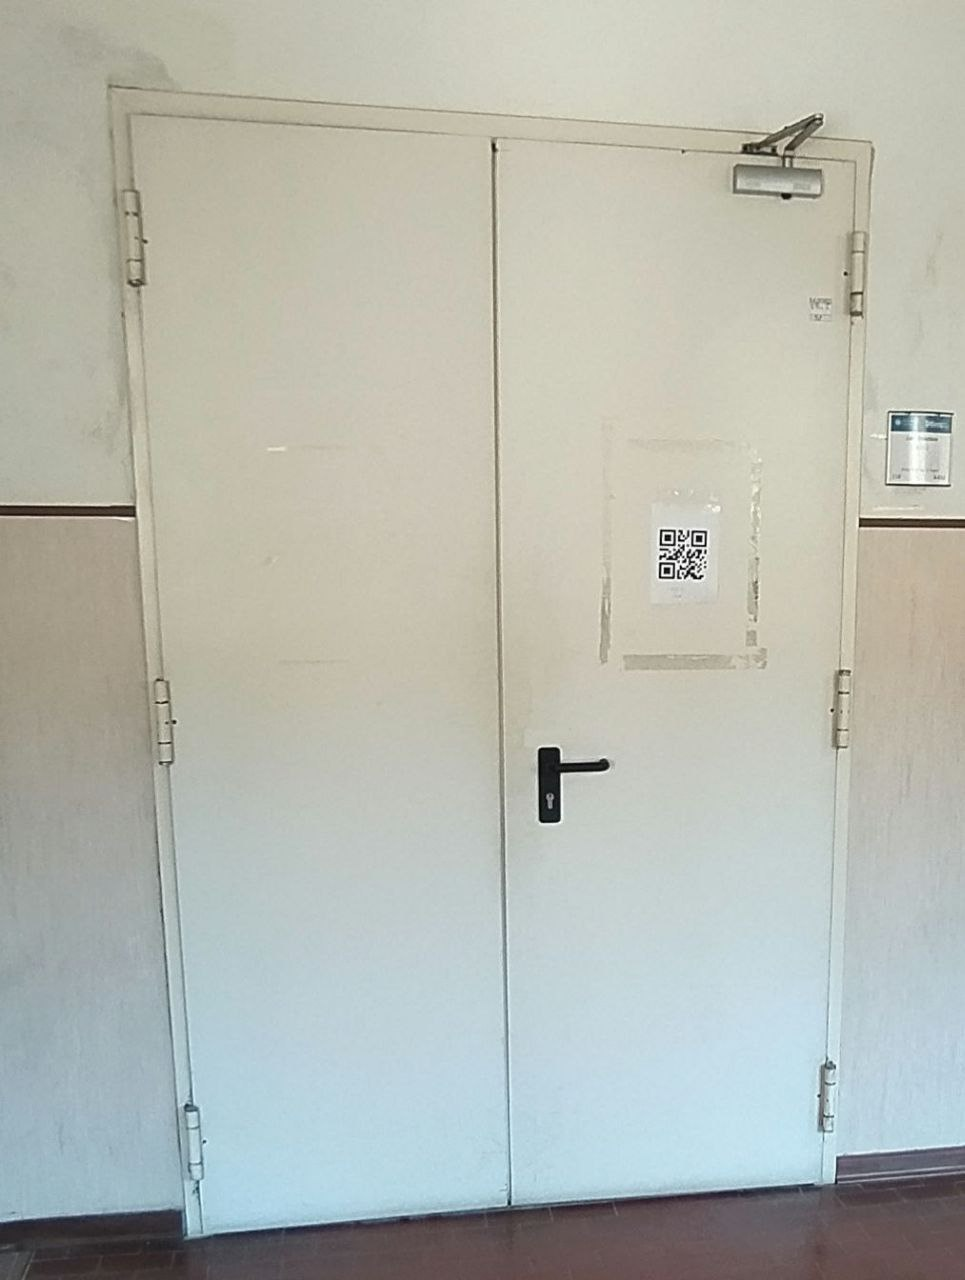
\includegraphics[width=0.6\columnwidth]{chapters/architecture/images/door-qr-codes.jpg}
    \caption{Example of intended arrangement of QR codes placed directly on the points of interest (a door, in this case).}
    \label{fig:door-qr-codes}
\end{figure}
